% !TeX spellcheck = <none>
\documentclass[a4paper,11pt]{article}
%Safely ignore everything until the sign DOCUMENT START HERE
\usepackage[]{graphicx}
\usepackage[]{color}
\usepackage{alltt}
\usepackage{amsmath}
\usepackage{algorithm}
\usepackage[toc,page]{appendix}
\usepackage[noend]{algpseudocode}
\usepackage[colorlinks,linkcolor=blue,anchorcolor=red,citecolor=green]{hyperref}%%%%%%
%\usepackage{subfigure}
\usepackage{subcaption}
\usepackage{array}
\usepackage[]{mcode}
\usepackage{booktabs}
\usepackage{amssymb}
\usepackage{listings}
%\usepackage[bitstream-charter]{mathdesign}
\usepackage[colorlinks,linkcolor=blue,anchorcolor=red,citecolor=green]{hyperref}
\usepackage{fancyhdr}
\usepackage{datetime}
\usepackage{amsmath}
\usepackage{graphicx}
    \providecommand{\tightlist}{%
	\setlength{\itemsep}{0pt}\setlength{\parskip}{0pt}}
\usepackage{graphicx}
\usepackage[section]{placeins}
\usepackage{geometry}
\usepackage{chngcntr}
\usepackage{tikz}
\renewcommand{\floatpagefraction}{.9}%
\setlength\parindent{0pt}
\usetikzlibrary{fit,positioning,arrows,automata}
\DeclareMathOperator*{\argmin}{arg\,min} 
\DeclareMathOperator*{\argmax}{arg\,max} 
\DeclareMathOperator{\E}{\mathbb{E}}
\graphicspath{ {images/} }
\counterwithout{figure}{section}
\geometry{left=2.0cm,right=2.0cm,top=2.5cm,bottom=2.5cm}
\numberwithin{equation}{section}
%\usepackage{hyperref}
%\usepackage{sectsty}
%\usepackage[T1]{fontenc}
\IfFileExists{upquote.sty}{\usepackage{upquote}}{}

%For R code visualization
\makeatletter
\def\maxwidth{ %
	\ifdim\Gin@nat@width>\linewidth
	\linewidth
	\else
	\Gin@nat@width
	\fi
}
\makeatother

\definecolor{fgcolor}{rgb}{0.345, 0.345, 0.345}
\newcommand{\hlnum}[1]{\textcolor[rgb]{0.686,0.059,0.569}{#1}}%
\newcommand{\hlstr}[1]{\textcolor[rgb]{0.192,0.494,0.8}{#1}}%
\newcommand{\hlcom}[1]{\textcolor[rgb]{0.678,0.584,0.686}{\textit{#1}}}%
\newcommand{\hlopt}[1]{\textcolor[rgb]{0,0,0}{#1}}%
\newcommand{\hlstd}[1]{\textcolor[rgb]{0.345,0.345,0.345}{#1}}%
\newcommand{\hlkwa}[1]{\textcolor[rgb]{0.161,0.373,0.58}{\textbf{#1}}}%
\newcommand{\hlkwb}[1]{\textcolor[rgb]{0.69,0.353,0.396}{#1}}%
\newcommand{\hlkwc}[1]{\textcolor[rgb]{0.333,0.667,0.333}{#1}}%
\newcommand{\hlkwd}[1]{\textcolor[rgb]{0.737,0.353,0.396}{\textbf{#1}}}%
\let\hlipl\hlkwb

\usepackage{framed}
\makeatletter
\newenvironment{kframe}{%
	\def\at@end@of@kframe{}%
	\ifinner\ifhmode%
	\def\at@end@of@kframe{\end{minipage}}%
\begin{minipage}{\columnwidth}%
	\fi\fi%
	\def\FrameCommand##1{\hskip\@totalleftmargin \hskip-\fboxsep
		\colorbox{shadecolor}{##1}\hskip-\fboxsep
		% There is no \\@totalrightmargin, so:
		\hskip-\linewidth \hskip-\@totalleftmargin \hskip\columnwidth}%
	\MakeFramed {\advance\hsize-\width
		\@totalleftmargin\z@ \linewidth\hsize
		\@setminipage}}%
{\par\unskip\endMakeFramed%
	\at@end@of@kframe}
\makeatother

\definecolor{shadecolor}{rgb}{.97, .97, .97}
\definecolor{messagecolor}{rgb}{0, 0, 0}
\definecolor{warningcolor}{rgb}{1, 0, 1}
\definecolor{errorcolor}{rgb}{1, 0, 0}
\definecolor{mygrey}{rgb}{0.172,0.172,0.172}
\newenvironment{knitrout}{}{} % an empty environment to be redefined in TeX

\fancyhf{}
\renewcommand{\headrulewidth}{0pt}
\fancyhf[HR]{\textcolor{mygrey}{First Interim Report}}
\pagestyle{plain}



\newcommand*{\captionsource}[2]{%
	\caption[{#1}]{%
		#1%
		\\\hspace{\linewidth}%
		\textbf{Source:} #2%
	}%
}


%DOCUMENT STARTS HERE!!!!!!

\begin{document}
	\title{%
		\textbf{Software - Logic Simulator Project
		} \\
		\Large First interim report\\
	}
	\date{Easter Term 2018}
	\author{S.~Arulselvan, F.~Freddi, A.~I.~Lam}
	\maketitle
	\thispagestyle{fancy}
	
	
	\lstset{aboveskip=\medskipamount}
	
	\section{Introduction}
This report introduces the reader to the general approach to the logic simulator problem. In the first few sessions of the projects we described the EBNF syntax of our logic simulator and we identified the possible semantic errors that might arise, considering how these should be handled. Two examples of how some of the most common circuit designs are represented using definition files consistent with the defined syntax. The team {\huge \verb|<-| WHAT?}

\section{Teamwork}
{\huge TODO}Shrin add here: add a brief description of how we decided to split the work between us and which tasks we are expecting to take more time than the others. Add brief comment to the gantt chart and refer to it in the appendix

add comment on expected rework and margin of time kept in case something goes wrong

\section{Specification of the language}
\subsection{Error identification}
\subsubsection{Identification of syntax errors and EBNF }
The EBNF is the stucture defining what rules the description of our circuit need to conform to and when syntax errors are thrown.

\begin{lstlisting}[caption= EBNF of the logic syntax,captionpos=b]
capitalletter = "A" | "B" | "C" | "D" | "E" | "F" | "G" | "H" | "I" | "J" | "K" 
		  	  | "L" | "M" | "N" | "O" | "P" | "Q" | "R" | "S" | "T" | "U" | "V" 
		  	  | "W" | "X" | "Y" | "Z" ;
lowerletter= "a" | "b"	| "c" | "d" | "e" | "f" | "g" | "h" | "i" | "j" | "k" | "l" 
		   | "m" | "n" | "o" | "p"	| "q" | "r" | "s" | "t" | "u" | "v" | "w" | "x" 
		   | "y" | "z" ;
digit = "0" | "1" | "2" | "3" | "4" | "5" | "6" | "7" | "8" | "9" ;

structure=devicelist,connectionlist,monitorlist,"END";

deviceslist= "DEVICE" , { devicedef } ;
devicedef= devicetype, device, { "," , device} , ";" ;
devicetype= capitalletter, {capitalletter};
device=devicename, [ "(" , digit , { digit } , ")" ];
devicename=(lowerletter | capitalletter), { lowerletter | capitalletter | digit };

connectionlist="CONNECT", {connection};
connection= output "->",input,{input},";";
input=devicename,".",capitalletter,{ capitalletter | digit };  
output=decivename, [".", capitalletter, {capitalletter}];

monitorlist="MONITOR", output, { "," , output};
\end{lstlisting}

\subsubsection{Identification of semantic errors} \label{ident_sem_error}
Considering the EBNF syntax design, further types of semantic errors can be identified:
\begin{enumerate}
	\tightlist
	\item a set of capital letters given for \textit{devicetype} is not a valid recognised \textit{devicetype}
	\item a device name is used more than once.
	\item the device name corresponds to a keyword or to a device type (considered case insensitive)
	\item a device is defined with parameters when the devicet type does not allow it (e.g.~XOR(5))
	\item a device is defined with parameters out of the parameter range (e.g.~SWITCH(4))
	\item multiple outputs going to the same input
	\item an input is not mentioned in the connections
	\item input index to a device must be less than or equal to the number of inputs initialised in DEFINE
	\item input/output name in CONNECT does not match the possible inputs of the device type
	\item in CONNECT and MONITOR, the \textit{devicename} has not been defined in DEFINE
	\item the same signal is monitored twice
\end{enumerate}

\subsection{Error handling}
Our approach to error handling starts from the syntax errors. If a syntax error is found, it is output and the parsing is continued on the rest of the file starting from the next semicolumn checking for the remaining syntax errors. If no syntax errors are found, we move to semantic error checking.
\subsubsection{Syntax errors}
All the syntax error are approached similarly displaying “SYNTAX ERRORS” followed by the line number, the involved code and an arrow underneath indicating where in line syntax error has occurred. Example:

\begin{lstlisting}
SYNTAX ERROR   Line 42: SWITCH 5n2;
                               ^
\end{lstlisting}
\subsubsection{Semantic errors}
Each type of semantic error is handled individually and, despite not being mentioned in the table, line number and the code generating the error will be included at beginning of the message. For the error number, refer to Section \ref{ident_sem_error}.

\begin{center}
	\begin{tabular}{l l}
		\hline
		\textbf{Error \#} & \textbf{Handling} \\ 
		\hline
		1 & Invalid device type: ``devicetype'' \\ 
		2 & Device name ``devicename'' was already used in line ``line''  \\ 
		3 & Cannot use keyword, ``devicename'', as a device name \\ 
		4 & ``devicetype'' type devices do not take parameters   \\ 
		5& SWITCH type device can only take 0 or 1 as parameter \\
		6 & Input ``input'' was already used in line “line”  \\
		7 & Input {``input''} was never used   \\
		8 & ``input'' cannot be used the ``num\_inputs'' input ``devicename'' device  \\
		9 & ``input''/``output'' is not valid for ``devicetype'' device ``devicename''   \\ 
		10 & Undefined device name:  ``devicename''  \\ 
		11 & ``signal'' is already monitored: line ``line'' \\
	\end{tabular}
	\captionof{table}{Error messages for each type of possible semantic error identified}
	\label{bandwidth-efficiency}
\end{center}

\section{Example definition files}
Two circuits are given in Figures \ref{fig:example1} and \ref{fig:example2},
by circuit diagrams and by the language defined above. 

\begin{figure}[htbp]
  \begin{subfigure}{\textwidth}
    \centering
    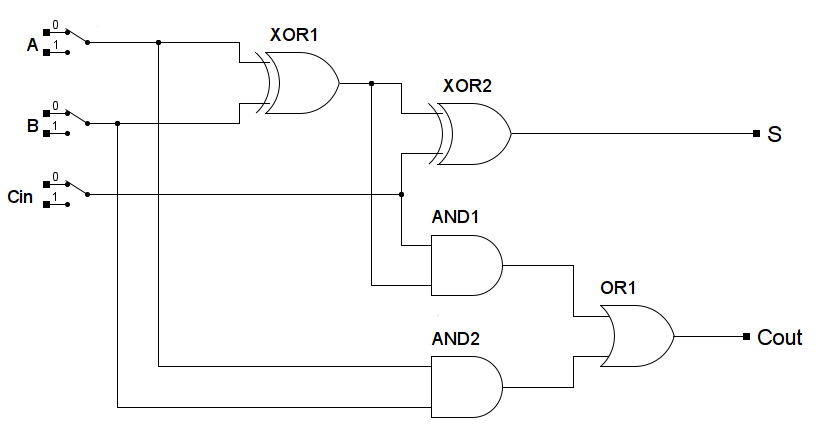
\includegraphics[scale=.33]{examples/fulladder.png}
    \caption{Circuit diagram for a full adder}
  \end{subfigure}
  \begin{subfigure}{\textwidth}
    \lstinputlisting{examples/fulladder.circuit}
    \caption{Full adder described by our language}
  \end{subfigure}
  \caption{A full adder, described equivalently by a standard circuit
    diagram and by our language.}
  \label{fig:example1}
\end{figure}

\begin{figure}[htbp]
  \begin{subfigure}{\textwidth}
    \centering
    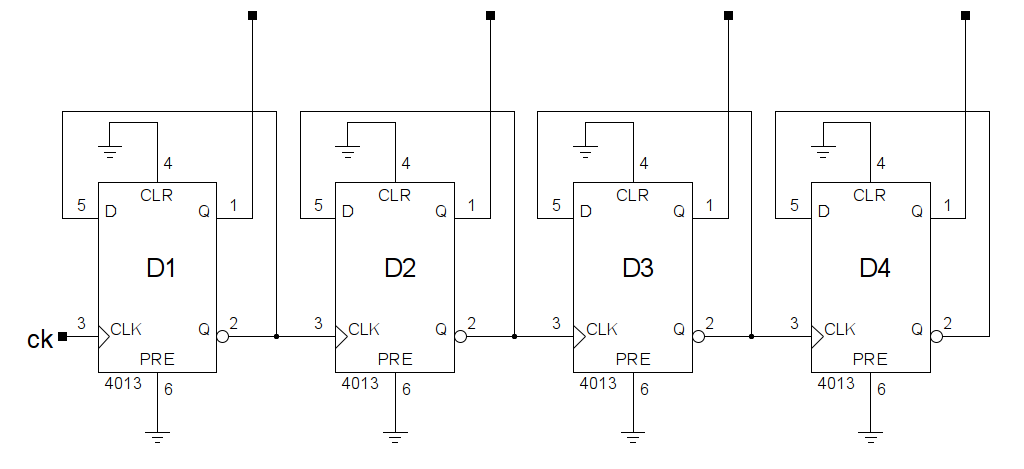
\includegraphics[scale=.33]{examples/ripplecounter.png}
    \caption{Circuit diagram for a ripple counter}
  \end{subfigure}
  \begin{subfigure}{\textwidth}
    \lstinputlisting{examples/ripplecounter.circuit}
    \caption{Ripple counter described by our language}
  \end{subfigure}
  \caption{A 4-bit ripple counter. Note that the circuit diagram is
    slightly simplified by implementing \texttt{gnd} directly as
    ground instead of a switch set to \texttt{0}, to avoid clutter
    in the diagram.}
  \label{fig:example2}
\end{figure}
\clearpage % outputs all floats


\begin{appendices} \label{app}
	\section{Gantt chart}
	{\huge TODO}Shrin add here
\end{appendices}

\end{document}
